\section{Planning Cost Functions}
\label{sec:cost}
In this section we present three different kinds of planning cost functions, each expecting different kinds of user input.

%%SL.10.15: Don't leave dangling sections like this without any text. Add a transition here to explain what this section is for and what comes next.

\subsection{Pixel-Distance based Cost}
\label{subsec:pixel_dist_cost}
A convenient way to define a robot task is by choosing one or more pixels in the robot's camera view and choosing a destination where each pixel should be moved. For example, the user might select a pixel on an object and ask the robot to move it 10 cm to the left. The advantages of this type of task definition are that success can be measured quantitatively in a straight-forward way, as detailed in section \ref{sec:experiments}.
%%SL.10.15: I think this needs more justification and motivation.

% Formally, the user specifies $P$ source pixel locations $\pixel_0^{(1)}, \dots, \pixel_0^{(P)}$ in the initial image $I_0$, and $P$ goal locations $\goal^{(1)}, \dots, \goal^{(P)}$. The source and goal pixel locations are denoted by the coordinates $(x_d^{(i)}, y_d^{(i)})$ and $(x_g^{(i)}, y_g^{(i)})$. Given a goal, the robot plans for a sequence of actions $\action_{1:T}$ over $T$ time steps, where $T$ is the planning horizon. For this type of task definition the problem is formulated as the minimization of a cost function $c$ which depends on the predicted pixel positions $d_t^{(j)}$. The planner makes use of a learned model that predicts a distribution over the pixel position by internally predicting pixel transformations. 
 
Given a distribution over pixel positions $P_0$ at time $t = 0$, the model predicts distributions over its positions $P_t$ at time $t \in \{ 1, \dots, T \}$. One way of defining the cost per time-step $c_t$ is by using the expected euclidean distance to the goal point $d_g$, which is straight-forward to calculate from $P_t$ and $g$, as follows:
 \begin{align}
c = \sum_{t = 1, \dots, T} c_t =  \sum_{t = 1, \dots, T} \mathbb{E}_{\hat{d}_{t} \sim P_{t}} \left[\|\hat{d}_{t} - d_{g}\|_2\right] 
 \label{eq:cost}
 \end{align}
The per time-step costs $c_t$ are summed together giving the overall planing objective $c$. 
%An alternative choice for the cost function is to evaluate $P_{t}$ at the position of the goal-point, which describes as how likely the model predicts an action sequence will hit the goal \emph{exactly}, we call this method \emph{goal-point evaluation}:
% \begin{align}
% c = \sum_{t = 1, \dots, T} P_t(g)
% \label{eq:goal_point_eval}
% \end{align}
The expected distance to the goal provides a smooth planning objective and enables longer-horizon tasks, since this cost function encourages movement of the designated objects into the right direction for each step of the execution, regardless of whether the goal-position can be reached within $T$ time steps or not. This cost also makes use of the uncertainty estimates of the predictor, when computing the expected distance to the goal. For multi-objective tasks with multiple designated pixels $d^{(i)}$ the costs are summed to together, and optionally weighted according to a scheme discussed in \autoref{subsec:reg_cost}.  

\subsection{Registration-Based Cost}
\label{subsec:reg_cost}
When using pixel distance-based cost functions it is necessary to know the initial locations $\pixel_0^{(1)}, \dots, \pixel_0^{(P)}$ at each time-step. To update the belief of where the target object currently is, we register the current image to the start and optionally also to a \emph{goal image}, where the designated pixels are marked by the user. Adding a goal-image can make visual-MPC more precise, since when the target object is close to the goal position, registration to the goal-image greatly improves the position estimate of the designated pixel. 

Crucially, the registration method we introduce is self-supervised, using the same exact data for training the video prediction model and the registration model. This allows both the predictor and registration model to continuously improve as the robot collects more data.

Before further detailing our learned registration system, we discuss a simple alternative approach for obtaining a cost-function for video-prediction based control: One na\"{i}ve approach could be to use the pixel-wise error, such as MSE, between a \emph{goal image} and the \emph{predicted image}. However there is a severe issue with this approach: When objects in the image are far from the position in the goal image (e.g., they do not overlap) there is no gradient signal with respect to changes in the actions, therefore optimization becomes impractical. 

\begin{figure}
	\centering
	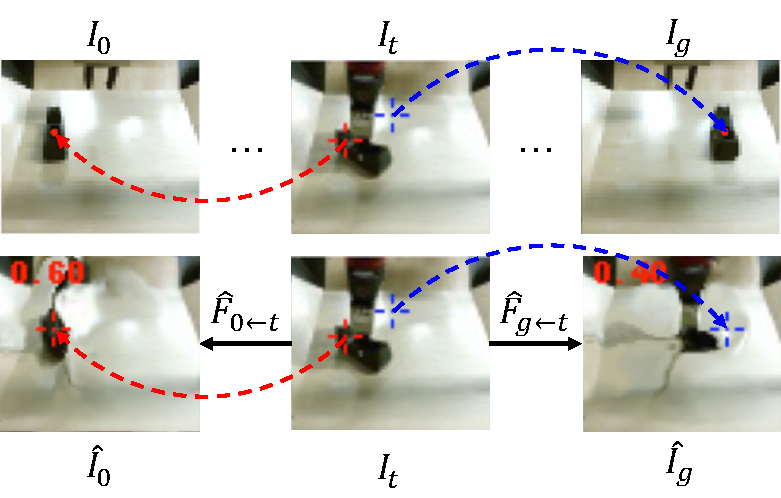
\includegraphics[width=0.8\linewidth]{images_rfr/registration_singletime.pdf}
	\caption{\small{Closed loop control is achieved by registering the current image $I_t$ globally to the first frame $I_0$ and the goal image $I_g$. In this example registration to $I_0$ succeeds while registration to $I_g$ fails since the object in $I_g$ is too far away.}
		\label{fig:reg_single}
	}
\end{figure}

\noindent \textbf{Test Time Procedure}
We will first describe the registration scheme at test time (see Figure~\ref{fig:registration_arch}(a)). We separately register the current image $I_t$ to the start image $I_0$ and to the goal image $I_g$ by passing it into the registration network $R$, implemented as a fully-convolutional neural network. The registration network produces a flow map $\hat{F}_{0 \leftarrow t} \in \mathbb{R}^{H \times W \times 2}$, a vector field with the same size as the image, that describes the relative motion for every pixel between the two frames.
\begin{align}
\hat{F}_{0 \leftarrow t} = R(I_t, I_0) &&
\hat{F}_{g \leftarrow t} = R(I_t, I_g)
\end{align}
The flow map $\hat{F}_{0 \leftarrow t}$ can be used to warp the image of the current time step $t$ to the start image $I_0$, and $\hat{F}_{g \leftarrow t}$ can be used to warp from $I_t$ to $I_g$ (see Figure \ref{fig:reg_single} for an illustration). There is no difference to the warping operation used in the video-prediction model, explained in section \ref{sec:model}, equation \ref{simple_dna}:
\begin{align}
\hat{I}_0 = \hat{F}_{0 \leftarrow t} \diamond  I_t &&
\hat{I}_g = \hat{F}_{g \leftarrow t} \diamond  I_t 
\end{align}
In essence for a current image $\hat{F}_{0 \leftarrow t}$ puts $I_t$ in correspondence with $I_0$, and $\hat{F}_{g \leftarrow t}$ puts $I_t$ in correspondence with $I_g$. The motivation for registering to both $I_0$ and $I_g$ is to increase accuracy and robustness. In principle, registering to either $I_0$ or $I_g$ is sufficient.

While the registration network is trained to perform a global registration between the images, we only evaluate it at the points $d_0$ and $d_g$ chosen by the user. This results in a cost function that ignores distractors. The flow map produced by the registration network is used to find the pixel locations corresponding to $d_0$ and $d_g$ in the current frame: 
\begin{align}
\hat{d}_{0,t} = d_0 + \hat{F}_{0 \leftarrow t}(d_0) &&
\hat{d}_{g,t} = d_g + \hat{F}_{g \leftarrow t}(d_g)
\label{eqn:warped_pos}
\end{align}


\begin{figure}[t!]
	\centering
	\begin{subfigure}[b]{0.35\linewidth}
		\centering
		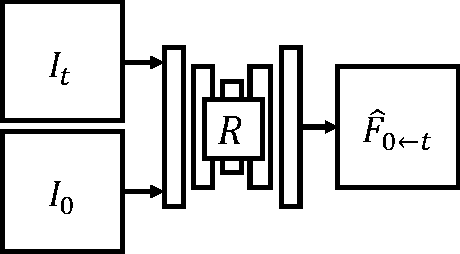
\includegraphics[width=\linewidth]{images_rfr/registration_test_start.pdf}\vspace{2.5mm}
		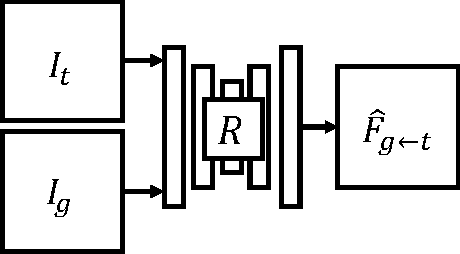
\includegraphics[width=\linewidth]{images_rfr/registration_test_goal.pdf}
		\caption{\small{Testing usage.}}
	\end{subfigure}
	\quad \quad
	\begin{subfigure}[b]{0.55\linewidth}
		\centering
		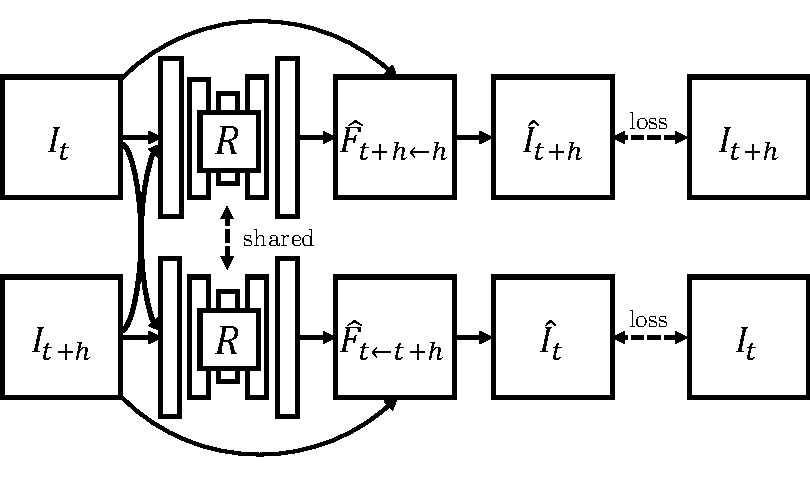
\includegraphics[width=\linewidth,trim={0 3mm 0 3mm},clip]{images_rfr/registration_train.pdf}
		\caption{\small{Training usage.}}
		\label{fig:discrete}
	\end{subfigure}
	\vspace{-1mm}
	\caption{\small{(a) At test time the registration network registers the current image $I_t$ to the start image $I_0$ (top) and goal image $I_g$ (bottom), inferring the flow-fields $\hat{F}_{0 \leftarrow t}$ and $\hat{F}_{g \leftarrow t}$. (b) The registration network is trained by warping images from randomly selected timesteps along a trajectory to each other.
	}}
	\label{fig:registration_arch}
\end{figure}

\begin{figure*}
	\centering
	\vspace{-0.1in}	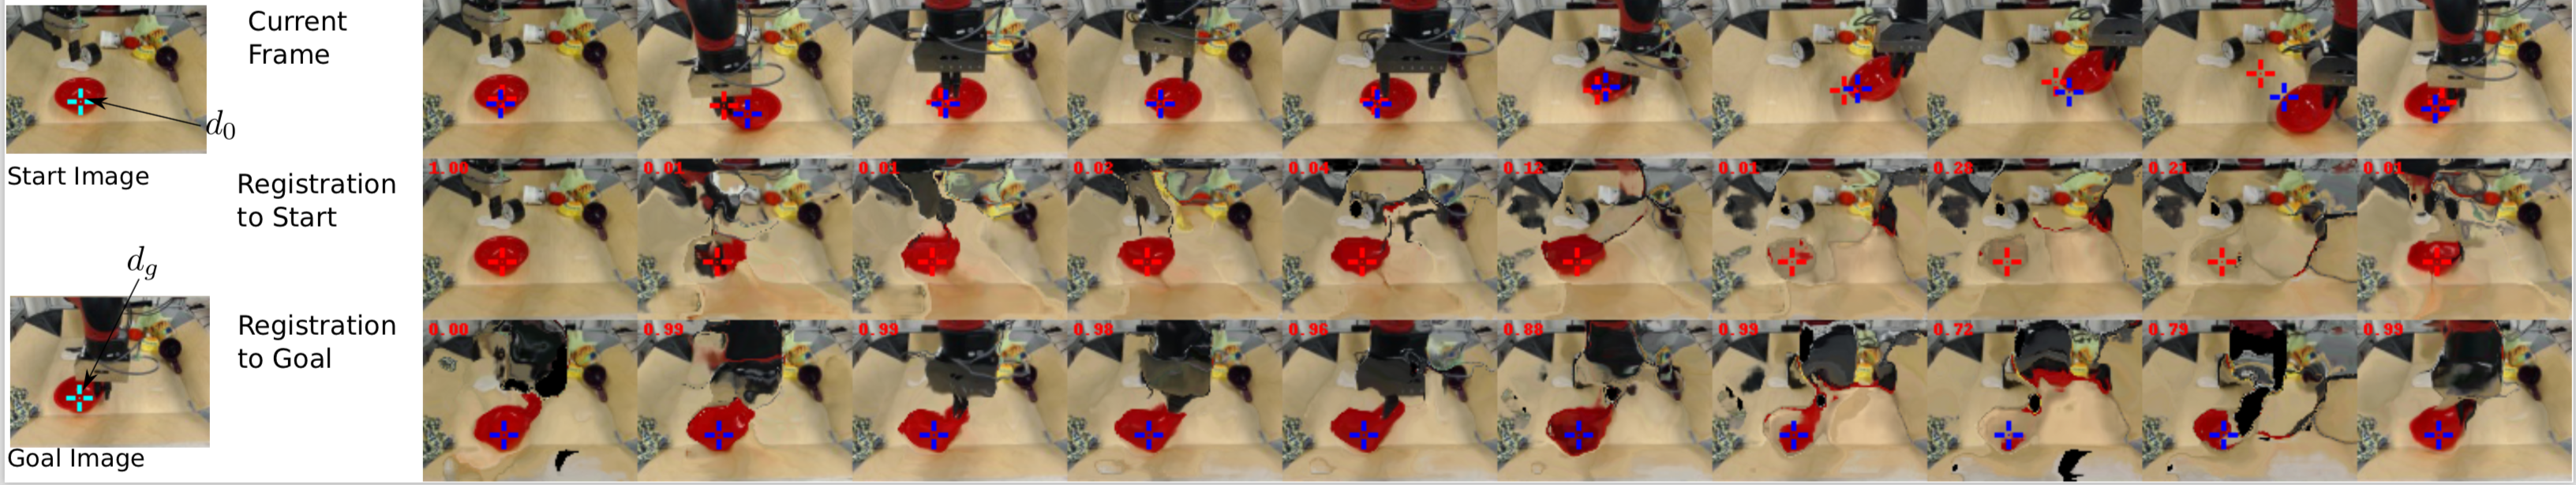
\includegraphics[width=1\linewidth]{images_rfr/reg_over_time.png}
	\caption{\small{Outputs of registration network. The first row shows the timesteps from left to right of a robot picking and moving a red bowl, the second row shows each image warped to the initial image via registration, and the third row shows the same for the goal image. A successful registration in this visualization would result in images that closely resemble the start- or goal image. In the first row, the locations where the designated pixel of the start image $d_0$ and the goal image $d_g$ are found are marked with red and blue crosses, respectively. It can be seen that the registration to the start image (red cross) is failing in the second to last time step, while the registration to the goal image (blue cross) succeeds for all time steps. The numbers in red, in the upper left corners indicate the trade off factors $\lambda$ between the views and are used as weighting factors for the planning cost. (Best viewed in PDF)}}
	\label{fig:tracking_overtime}
	\vspace{-0.2in}
\end{figure*}

For simplicity, we describe the case with a single designated pixel. In practice, instead of a single flow vector $\hat{F}_{0 \leftarrow t}(d_0)$ and $\hat{F}_{g \leftarrow t}(d_g)$, we consider a neighborhood of flow-vectors around $d_0$ and $d_g$ and take the median in the $x$ and $y$ directions, making the registration more stable.
\autoref{fig:tracking_overtime} visualizes an example tracking result while the gripper is moving an object.

\noindent \textbf{Registration-Based Pixel-Distance Cost}
Registration can fail when distances between objects in the images are large. During a trajectory, the registration to the first image typically becomes harder, while the registration to the goal image becomes easier. We propose a mechanism that estimates which image is registered correctly, allowing us to utilize only the successful registration for evaluating the planning cost. This mechanism gives a high weight $\lambda_i$ to pixel-distance costs $c_i$ associated with a designated pixel $\hat{d}_{i,t}$ that is tracked successfully and a low, ideally zero, weight to a designated pixel where the registration is poor. We propose to use the photometric distance between the true frame and the warped frame evaluated at $d_{0,i}$ and $d_{g,i}$ as an estimate for \emph{local} registration success. A low photometric error indicates that the registration network predicted a flow vector leading to a pixel with a similar color, thus indicating warping success. However this does not necessarily mean that the flow vector points to the correct location. For example, there could be several objects with the same color and the network could simply point to the wrong object. Letting $I_i(d_i)$ denote the pixel value in image $I_i$ for position $d_i$, and $\hat{I}_i(d_i)$ denote the corresponding pixel in the image warped by the registration function, we can define the general weighting factors $\lambda_i$ as:
\begin{align}
\lambda_i =  \frac{||I_i(d_i) - \hat{I_i}(d_i)||_2^{-1}}{\sum^N_j ||I_j(d_j) - \hat{I}_j(d_j)||^{-1}_2}.
\label{eqn:cost_avg}
\end{align}
where $\hat{I}_i = \hat{F}_{i \leftarrow t} \diamond I_t$. The MPC cost is computed as the average of the costs $c_i$ weighted by $\lambda_i$, where each $c_i$ is the expected distance (see equation \ref{eq:cost}) between the registered point $\hat{d}_{i,t}$ and the goal point $d_{g,i}$. Hence, the cost used for planning is $c = \sum_i \lambda_i c_i$.  In the case of the single view model and a single designated pixel, the index $i$ iterates over the start and goal image (and $N=2$).

The proposed weighting scheme can also be used with multiple designated pixels, as used in multi-task settings and multi-view models, which are explained in section \ref{sec:multiview}. The index $i$ then also loops over the views and indices of the designated pixels.

\noindent \textbf{Training Procedure}
The registration network is trained on the same data as the video-prediction model, but it does not share parameters with it.\footnote{in principle sharing parameters with the video-prediction model might be beneficial, however this is left for future work} Our approach is similar to the optic flow method proposed by \cite{meister2017unflow}. However, unlike this prior work, our method computes registrations for frames that might be many time steps apart, and the goal is not to extract optic flow, but rather to determine correspondences between potentially distant images. For training, two images are sampled at random times steps $t$ and $t+h$ along the trajectory and the images are warped to each other in both directions. 
\begin{align}
\hat{I}_{t} = \hat{F}_{t \leftarrow t +h} \diamond  I_{t+h} &&
\hat{I}_{t+h} = \hat{F}_{t+h \leftarrow t} \diamond  I_{t}
\end{align}
The network, which outputs $\hat{F}_{t \leftarrow t +h}$ and $\hat{F}_{t+h \leftarrow t}$, see Figure~\ref{fig:registration_arch} (b), is trained to minimize the photometric distance between $\hat{I}_t$ and $I_t$ and $\hat{I}_{t+h}$ and $I_{t+h}$, in addition to a smoothness regularizer that penalizes abrupt changes in the outputted flow-field. The details of this loss function follow prior work \cite{meister2017unflow}. We found that gradually increasing the temporal distance $h$ between the images during training yielded better final accuracy, as it creates a learning curriculum. The temporal distance is linearly increased from 1 step to 8 steps at 20k SGD steps. In total 60k iterations were taken.

The network $R$ is implemented as a fully convolutional network taking in two images stacked along the channel dimension. First the inputs are passed into three convolutional layers each followed by a bilinear downsampling operation. This is passed into three layers of convolution each followed by a bilinear upsampling operation (all convolutions use stride 1). By using bilinear sampling for increasing or decreasing image sizes we avoid artifacts that are caused by strided convolutions and deconvolutions.


\subsection{Classifier-Based Cost Functions}
\label{subsec:class_cost}
An alternative way to define the cost function is with a goal classifier. This type of cost function is particularly well-suited for tasks that can be completed in multiple ways. For example, for a task of rearranging a pair objects into relative positions, i.e. pushing the first object to the left of the second object, the absolute positions of the objects do not matter nor does the arm position. A classifier-based cost function allows the planner to discover any of the possible goal states. 

Unfortunately, a typical image classifier will require a large amount of labeled examples to learn, and we don't want to collect large datasets for each and every task. Instead, we aim to learn a goal classifier from only a few positive examples, using a meta-learning approach. A few positive examples of success are easy for people to provide and are the minimal information needed to convey a goal.

\newcommand{\task}{\mathcal{T}}
\newcommand{\data}{\mathcal{D}}
\newcommand{\obs}{\mathbf{o}}
\newcommand{\out}{y}
\newcommand{\posdata}{\data^+}
\newcommand{\testdata}{\data^\text{test}}
\newcommand{\loss}{\mathcal{L}}

Formally, we consider a goal classifier $\hat{\out} = f(\obs)$, where $\obs$ denotes the image observation, and $\hat{\out} \in [0,1]$ indicates the predicted probability of the observation being of a successful outcome of the task. Our objective is to infer a classifier for a new task $\task_j$ from a few positive examples of success, which are easy for a user to provide and encode the minimal information needed to convey a task. In other words, given a dataset $\posdata_j$ of $K$ examples of successful end states for a new task $\task_j$: $\data_j:=\{(\obs_k, 1) | k = 1...K\}_j$, our goal is to infer a classifier for task $\task_j$. 

\begin{figure}
    \centering
    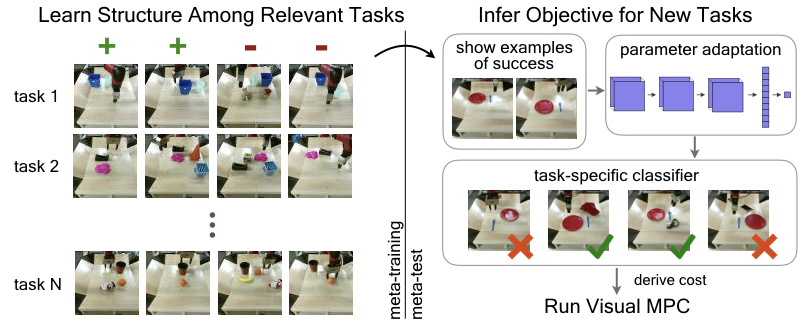
\includegraphics[width=0.48\textwidth]{images_cls/cls_fig.jpeg}
    \caption{\small We propose a framework for quickly specifying visual goals. Our goal classifier is meta-trained with positive and negative examples for diverse tasks (left), which allows it to meta-learn that some factors matter for goals (e.g., relative positions of objects), while some do not (e.g. position of the arm). At meta-test time, this classifier can learn goals for new tasks from a few of examples of success (right - the goal is to place the fork to the right of the plate). The cost can be derived from the learned goal classifier for use with visual MPC.}
    \label{fig:cls_fig}
    \vspace{-0.3cm}
\end{figure}

\noindent \textbf{Meta-Learning for Few-Shot Goal Inference:}
To solve the above problem, we propose learning a few-shot classifier that can infer the goal of a new task from a small set of goal examples, allowing the user to define a task from a few examples of success. To train the few-shot classifier, we first collect a dataset of both positive and negative examples for a wide range of tasks. We then use this data to learn how to learn goal classifiers from a few positive examples.
Our approach is illustrated in Figure~\ref{fig:cls_fig}.

We build upon model-agnostic meta-learning (MAML)~\cite{maml}, which learns initial parameters $\theta$ for model $f$ that can efficiently adapt to a new task with one or a few steps of gradient descent. Grant et al. \cite{caml} proposed an extension of MAML, referred to as concept acquisition through meta-learning (CAML), for learning to learn new concepts from positive examples alone. We apply CAML to the setting of acquiring goal classifiers from positive examples, using a meta-training data with both positive and negative examples. The result of the meta-training procedure is an initial set of parameters that can be used to learn new goal classifiers at test time.

\noindent \textbf{Test Time Procedure:}
At test time, the user provides a dataset $\posdata_j$ of $K$ examples of successful end states for a new task $\task_j$: $\data_j:=\{(\obs_k, 1) | k = 1...K\}_j$, which are then used to infer a task-specific goal classifier $C_j$. In particular, the meta-learned parameters $\theta$ are updated through gradient descent to adapt to task $\task_j$:

$$
C_j(\obs)
= f(\obs; \theta_j')
= f\big(\obs; \theta-\alpha \nabla_\theta \!\!\! \sum_{(\obs_n, \out_n)\in \posdata_j} \loss (\out_n, f(\obs_n; \theta)\big)
$$

where $\loss$ is the cross-entropy loss function, $\alpha$ is the step size, and $\theta'$ denotes the parameters updated through gradient descent on task $\task_j$.

During planning, the learned classifier $C_j$ takes as input an image generated by the video-prediction model and outputs the predicted probability of the goal being achieved for the task specified by the few examples of success. To convert this into a cost function, we treat the probability of success as the planning cost for that observation. To reduce the effect of false positives and mis-calibrated predictions, we use the classifier conservatively by thresholding the predictions so that reward is only given for confident successes. Below this threshold, we give a reward of 0 and above this threshold, we provide the predicted probability as the reward.


\noindent \textbf{Train time procedure}
During meta-training, we explicitly train for the ability to infer goal classifiers for the set of training tasks, $\{ \task_i \}$. We assume a small dataset $\data_i$ for each task $\task_i$, consisting of both positive and negative examples: $\data_i:= \{(\obs_n,\out_n) | n=1...N \}_i$. To learn the initial parameters $\theta$, we optimize the following objective:

$$
\min_\theta \sum_i \sum_{(\obs_n, y_n) \in \testdata_i} \loss(\out_n, f(\obs_n; \theta_i')) 
$$

We optimize this objective using Adam~\cite{ADAM} on the initial parameters $\theta$. In our experiments, our classifier is represented by a convolutional neural network, consisting of three convolutional layers, each followed by layer normalization and a ReLU non-linearity. After the final convolutional layer, a spatial soft-argmax operation extracts spatial feature points, which are then passed through fully-connected layers.

\subsection{When to use which Cost Function?}
\label{subsec:cost_discuission}

We have introduced three different kinds of cost functions, pixel-distance based cost functions with and without registration, as well as classifier-based cost functions. Here we discuss the relative strengths and weaknesses of each of them.

Pixel-distance based cost functions have the advantage that they allow moving objects precisely to target locations. Further, they do not the user to provide an image of the goal, creating a simple and easy interface for specifying goals. The pixel-distance based cost function also has a high degree of robustness against distractor objects and clutter since the optimizer can ignore the values of other pixels; this is an important feature when targeting diverse real-world environments.
By incorporating an image of the goal, we can add a registration mechanism to allow for more robust closed-loop control, at the cost of a more significant burden on the user.

The classifier-based cost function allows for solving more abstract tasks where the absolute positions of an object can be irrelevant, such as position a cup in front of a plate, irrespective of where the plate is.  Providing a few example images takes more effort than specifying pixel locations but allows a broader range of goal sets to be specified.

%%SL.10.15: This is rather... terse. Maybe that's OK not to be too verbose, but the section somehow feels a bit unfinished.
%%CF.11.20: I agree. I made a bunch of changes to make it less terse.
